\documentclass{article} % For LaTeX2e
\usepackage{nips13submit_e,times}
\usepackage{hyperref}
\usepackage{url}
\usepackage{graphicx}
\usepackage{subfig}
\usepackage[section]{placeins}

\title{Extracting Food Entities from Yelp Reviews}


\author{
Rahul Ramakrishna \\
Department of Computer Science\\
University of Massachusetts Amherst\\
\texttt{rahulram@cs.umass.edu} \\
}

% The \author macro works with any number of authors. There are two commands
% used to separate the names and addresses of multiple authors: \And and \AND.
%
% Using \And between authors leaves it to \LaTeX{} to determine where to break
% the lines. Using \AND forces a linebreak at that point. So, if \LaTeX{}
% puts 3 of 4 authors names on the first line, and the last on the second
% line, try using \AND instead of \And before the third author name.

\newcommand{\fix}{\marginpar{FIX}}
\newcommand{\new}{\marginpar{NEW}}

%\nipsfinalcopy % Uncomment for camera-ready version

\begin{document}


\maketitle


\begin{abstract}

Many of the restaurants listed in yelp \footnote{\url{http://www.yelp.com/dataset_challenge/}} may not have the the latest updated menu. Its really hard for the user to figure out, which food item is served best in a given restaurant since, most of the menu cards are graphic images linked to external websites or have not been updated for a long time. Also, its very unlikely that all the menu items will be a special delicacy for a given restaurant. Thus, to fetch this information, its important to categorize various food entities mentioned by reviewers [1]. This will help us in ranking food items based on reviews for a given restaurant. 

To derieve any meaning information from users review about food items, we need to first build a high quality dictionary of food items. We use a semi-supervised method using various classfiers to classify whether a word is food item or not. Using this we infered some interseting insights into yelp dataset and found corelations between number of words in a give user review to average rating of the restaurant. We also got a accurate ranking of food items for a given restaurant.

%:Given plethora of yelp reviews, we need to classify whether the entity is a food related or not. In order to solve this classification problem, we need to build a basic test bed of words which are food related (+ve set) and non-food related words (-ve set). A manually created list of 30-40 examples would suffice, since low-dimensional dense vectors generalizes well than high-dimensional sparse vectors. [1,2]

%The text reviews are extracted and are to coagulated using a pre-processor which will process the reviews and purge unrelated information. For example, phone numbers would be replaced to string phone\_number. The processed reviews will be fed to the word2vectors \footnote{ \url{http://code.google.com/p/word2vec/ } } to generate vectors for each of the words and phrases. The vectors will be used passed as features to classification algorithms. Once, word vectors with their features are built along with manually curated list of +ve food entity and -ve food entities, various classification algorithms like SVM, Logistic Regression \footnote{ Libraries from \url{http://scikit-learn.org/}} will be used to classify and generate probabilities for a given entity to be food related or not. Precision and Recall metrics will be calibrated at P@50, P@100 \& P@500 on sorted list of words with higher probabilities.

%K-fold cross validation techniques will be applied to validate the pipeline and experiments will be performed on which classifying algorithm performs better. Once a high quality dictionary of food entities is built, we can later use this data to generate best dishes from a given restaurant or best food items from a given city by associating the food entities mentioned in review with ratings.

%As for future work, we can build dictionary of attributes from the restaurant reviews alone. For example, attributes like cleanliness, waiter-friendly, peaceful etc can be extracted. Also, we can extend this idea to embed recommendations during search \footnote{ \url{https://www.algolia.com/}}

\end{abstract}


\section{Related Work}



\section{Proposed Solution}


\begin{figure}[h]
  \begin{center}
    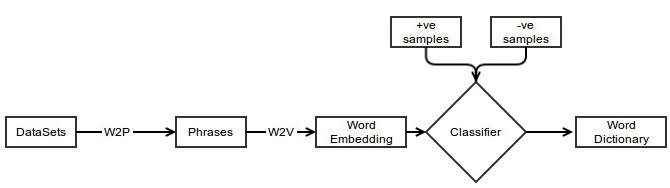
\includegraphics[scale=0.6]{ml.jpg}
    \label{fig:1}
    \caption{}
  \end{center}
\end{figure}


\section{Data Set}

Preliminary analysis of the dataset. After pre-processing the yelp reviews, based on reviews we have seggregated the reviews on Good (ratings 4 $\geq$  ),Ok (ratings 3-3.5) and Bad ( $<$ 3 )ratings. The following graph shows the distribution of these ratings

\begin{figure}[h]
  \begin{center}
    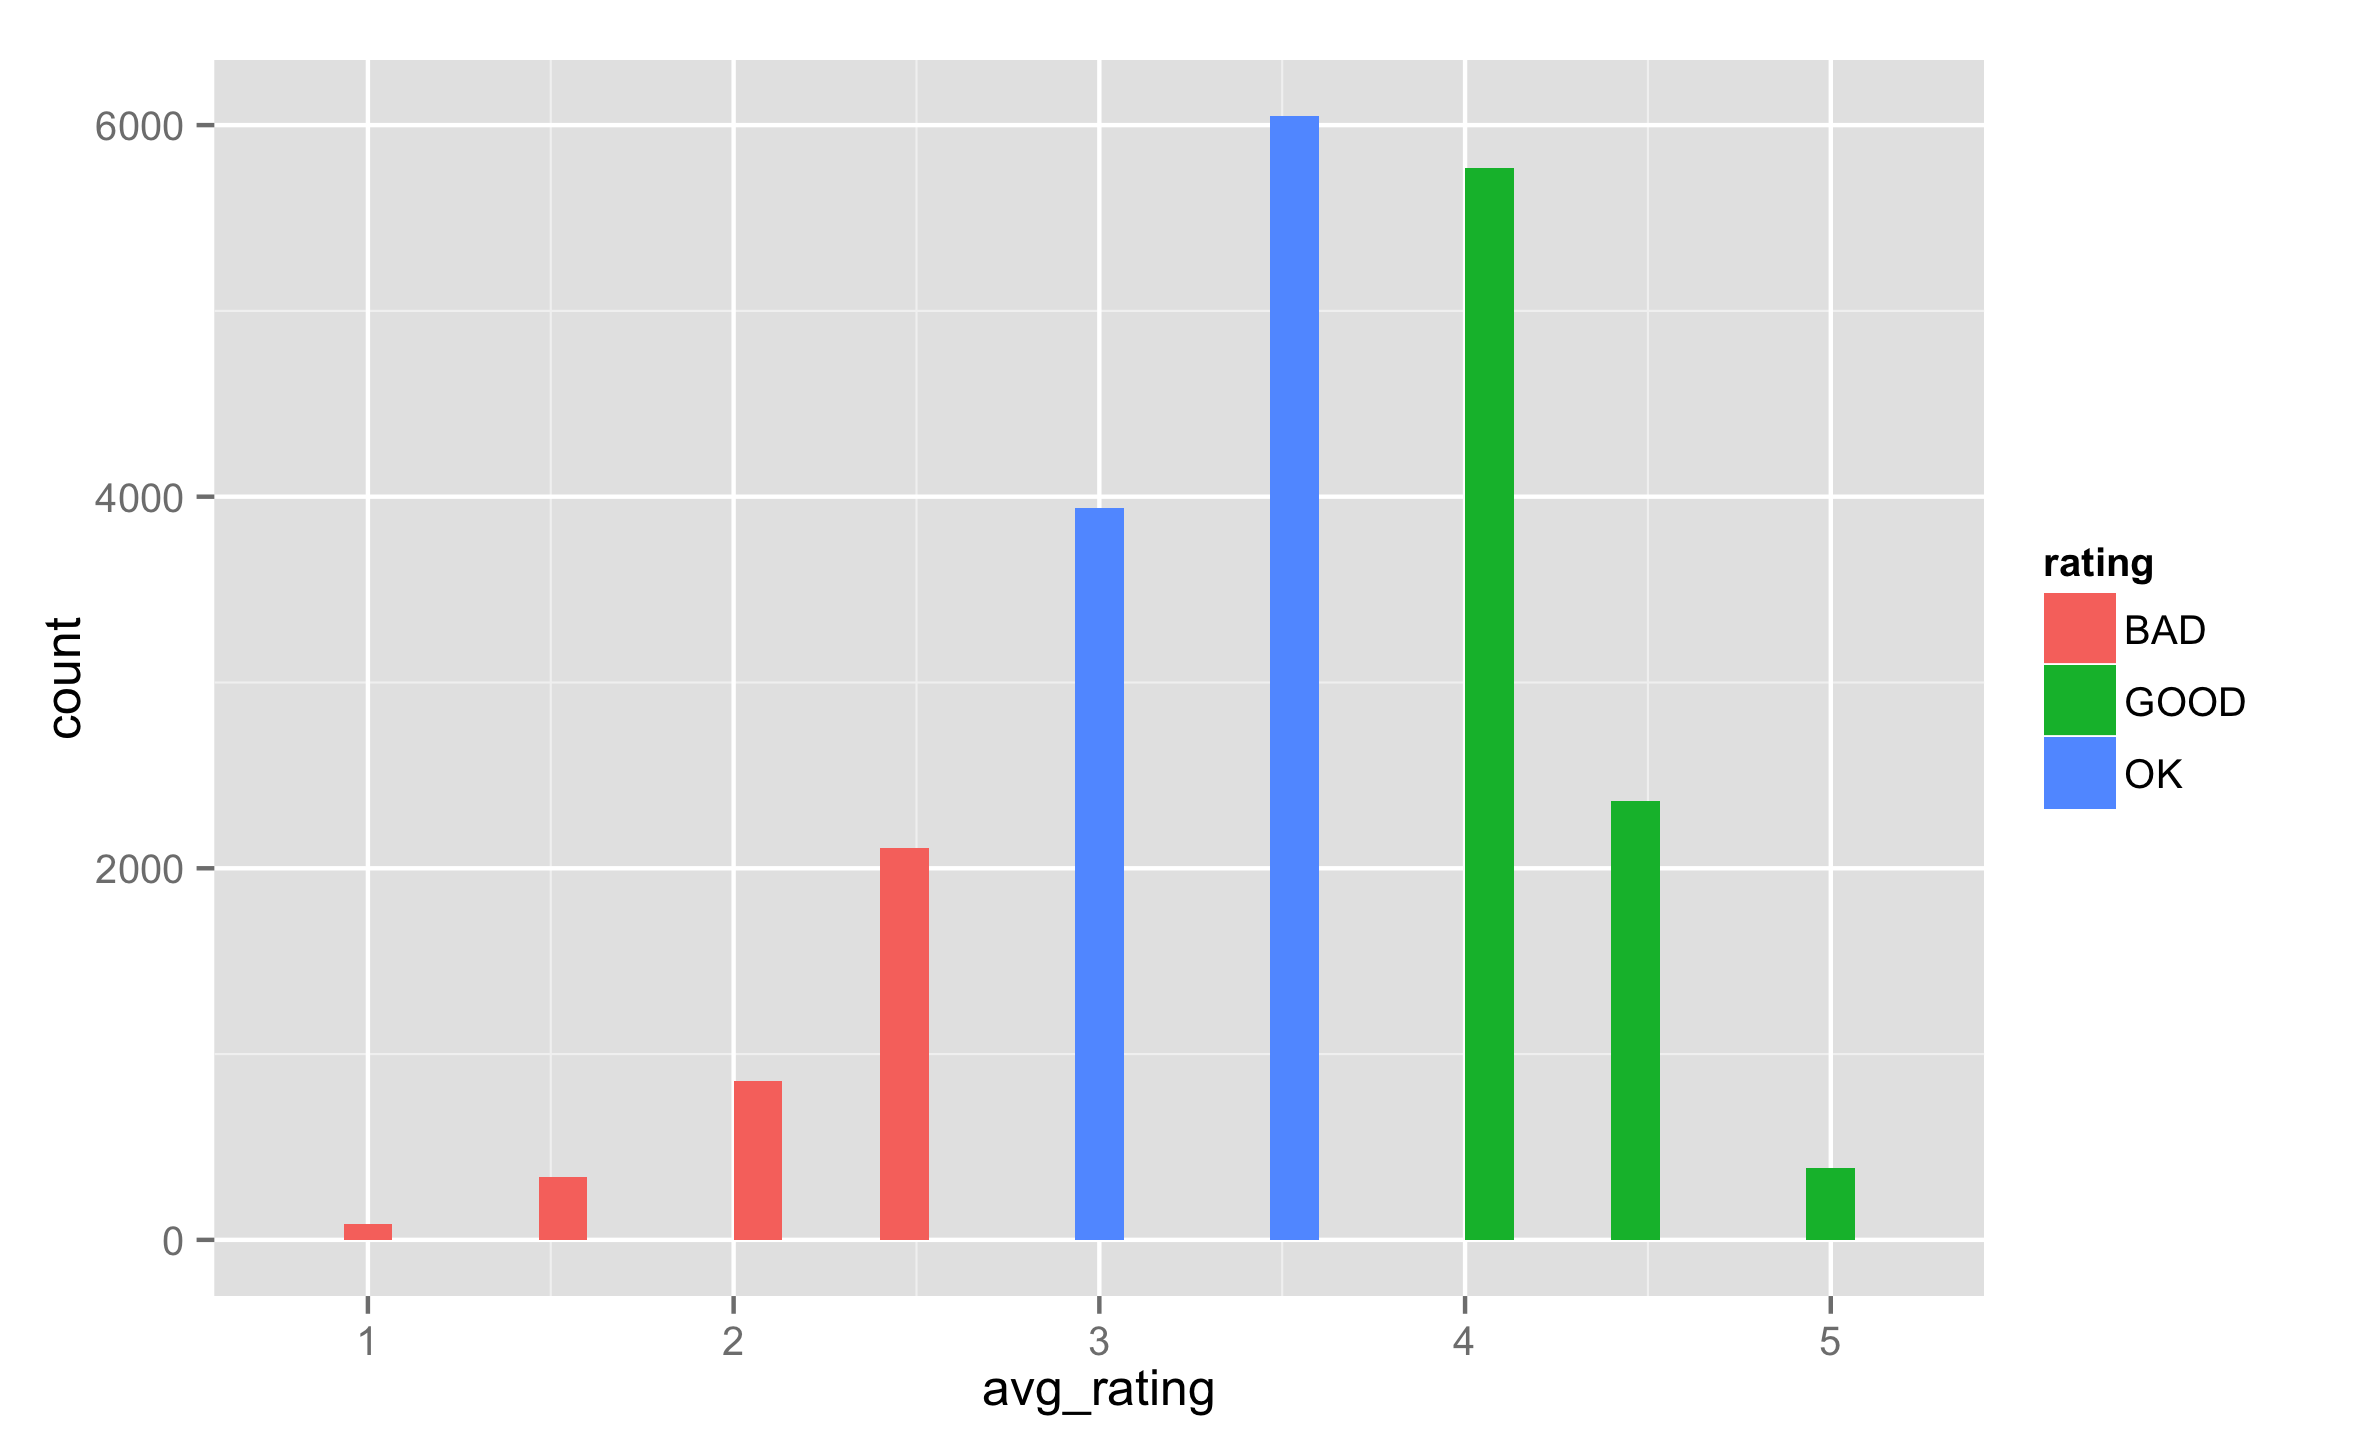
\includegraphics[scale=0.1]{./plots/avg-rating.png}
    \label{fig:}
    \caption{}
  \end{center}
\end{figure}


No of reviews 

\begin{figure}[h]
    \centering
    \subfloat[label 1]{{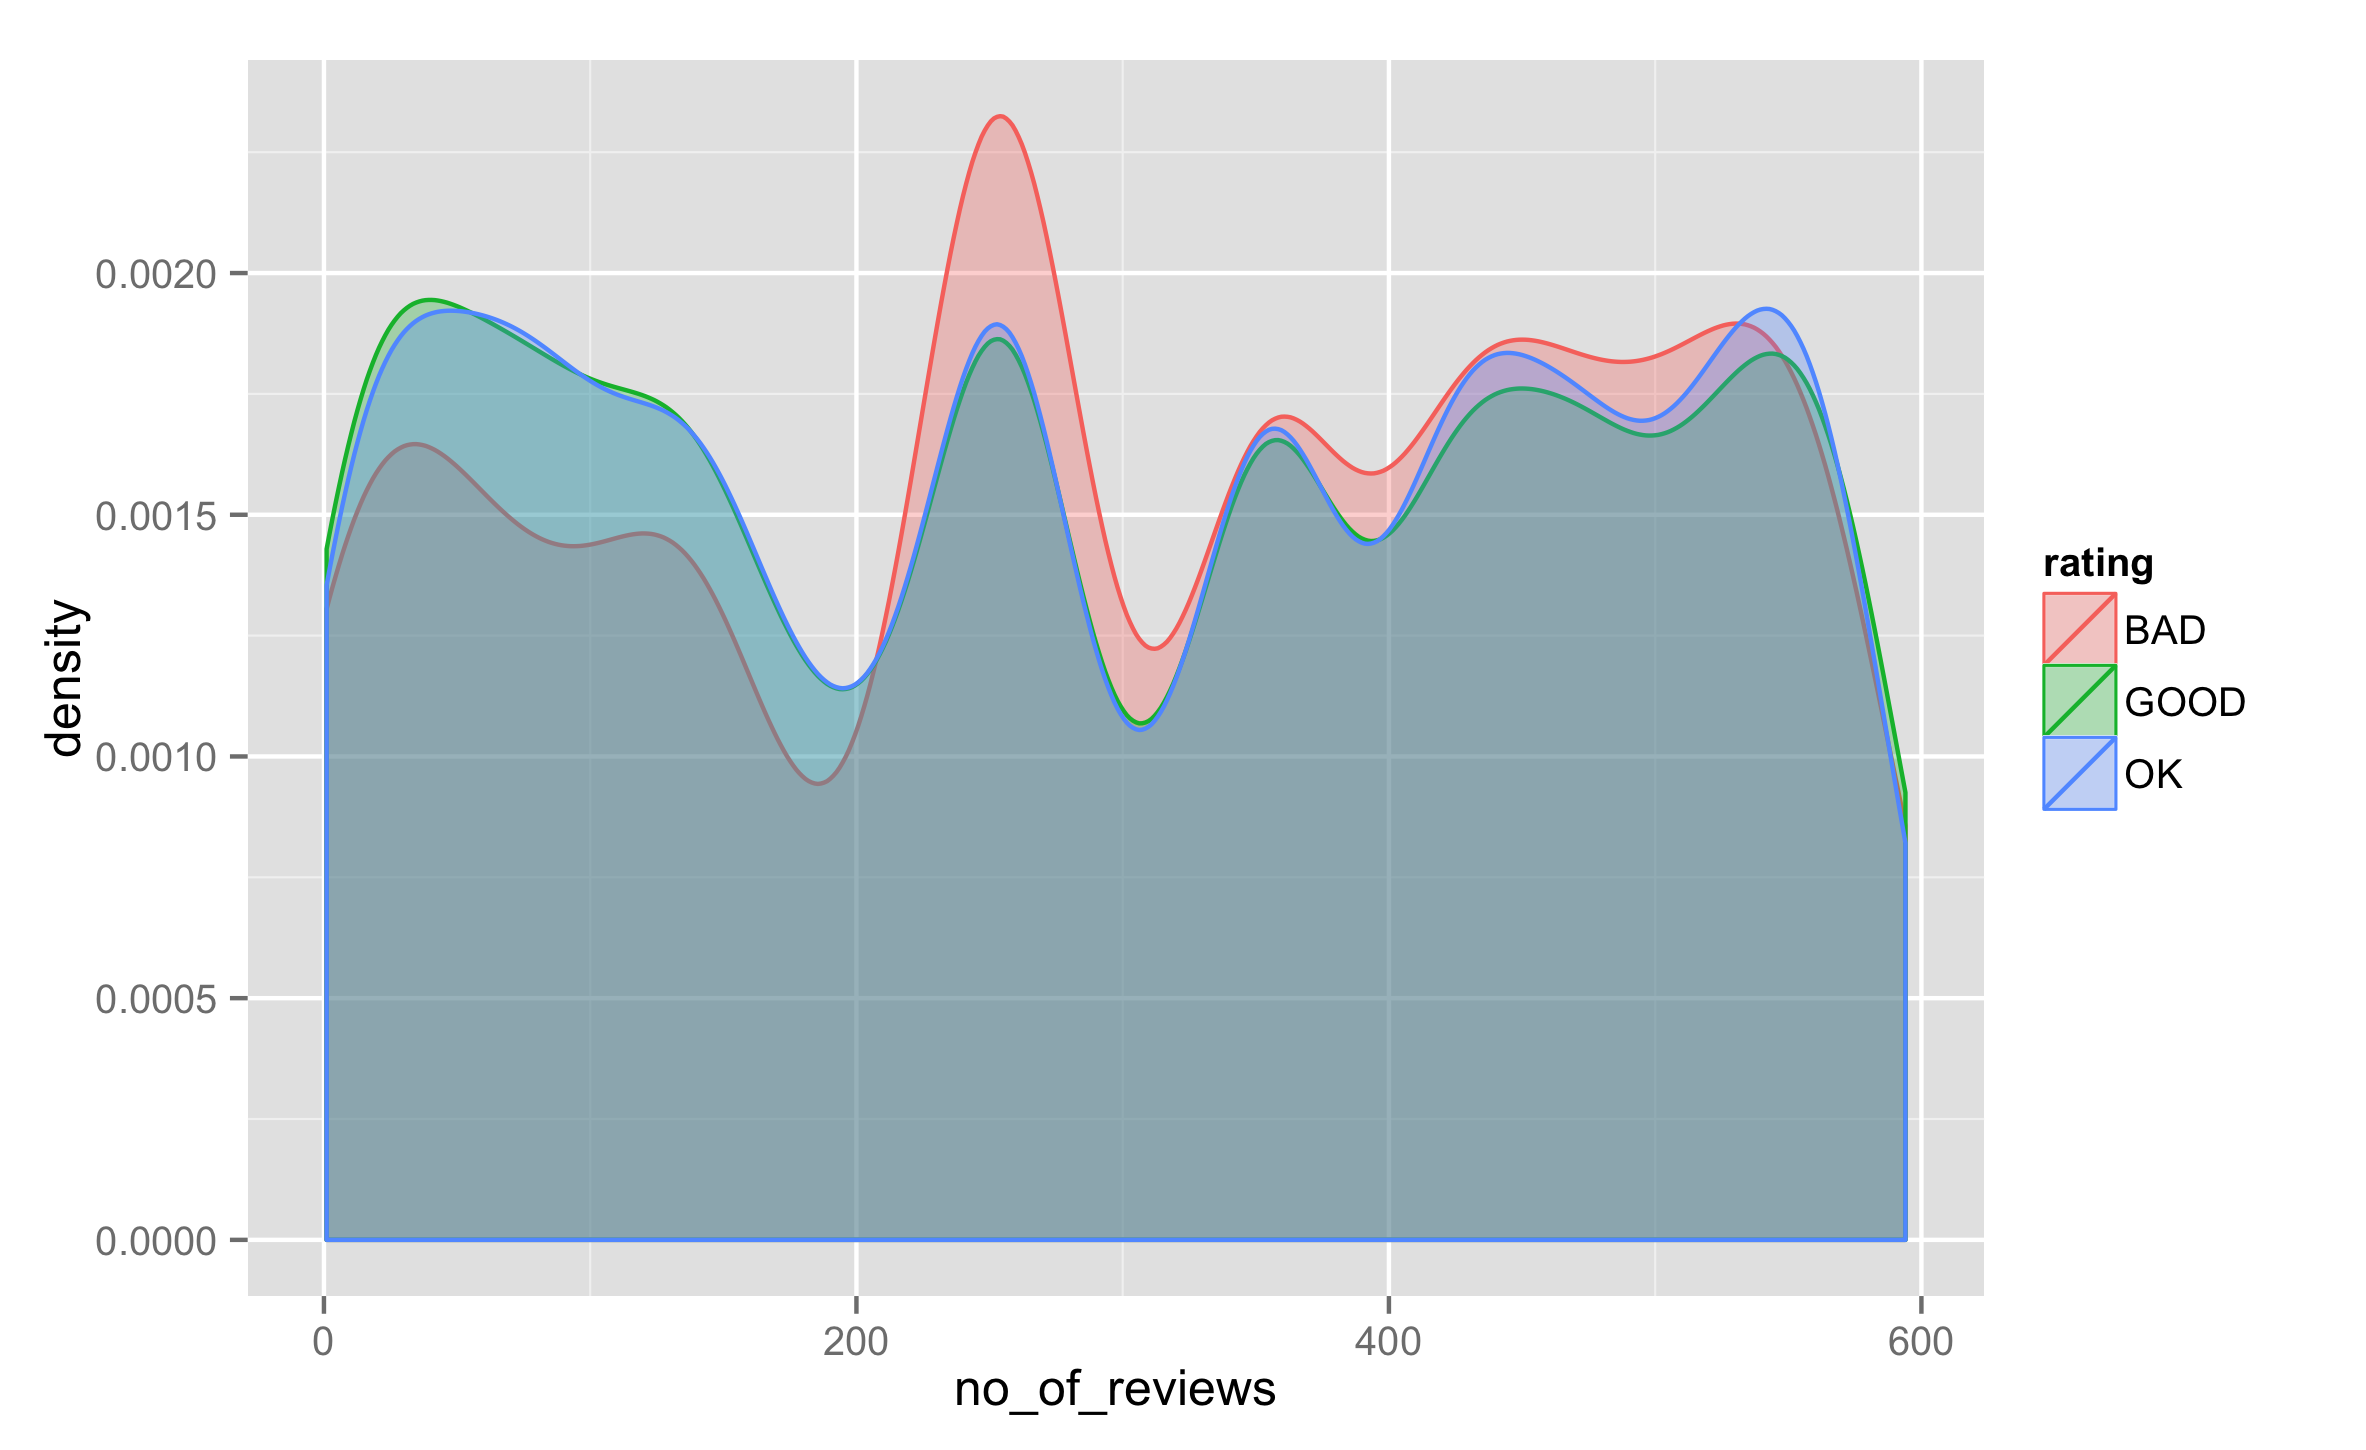
\includegraphics[width=6cm]{./plots/no-of-reviews.png} }}%
    \qquad
    \subfloat[label 2]{{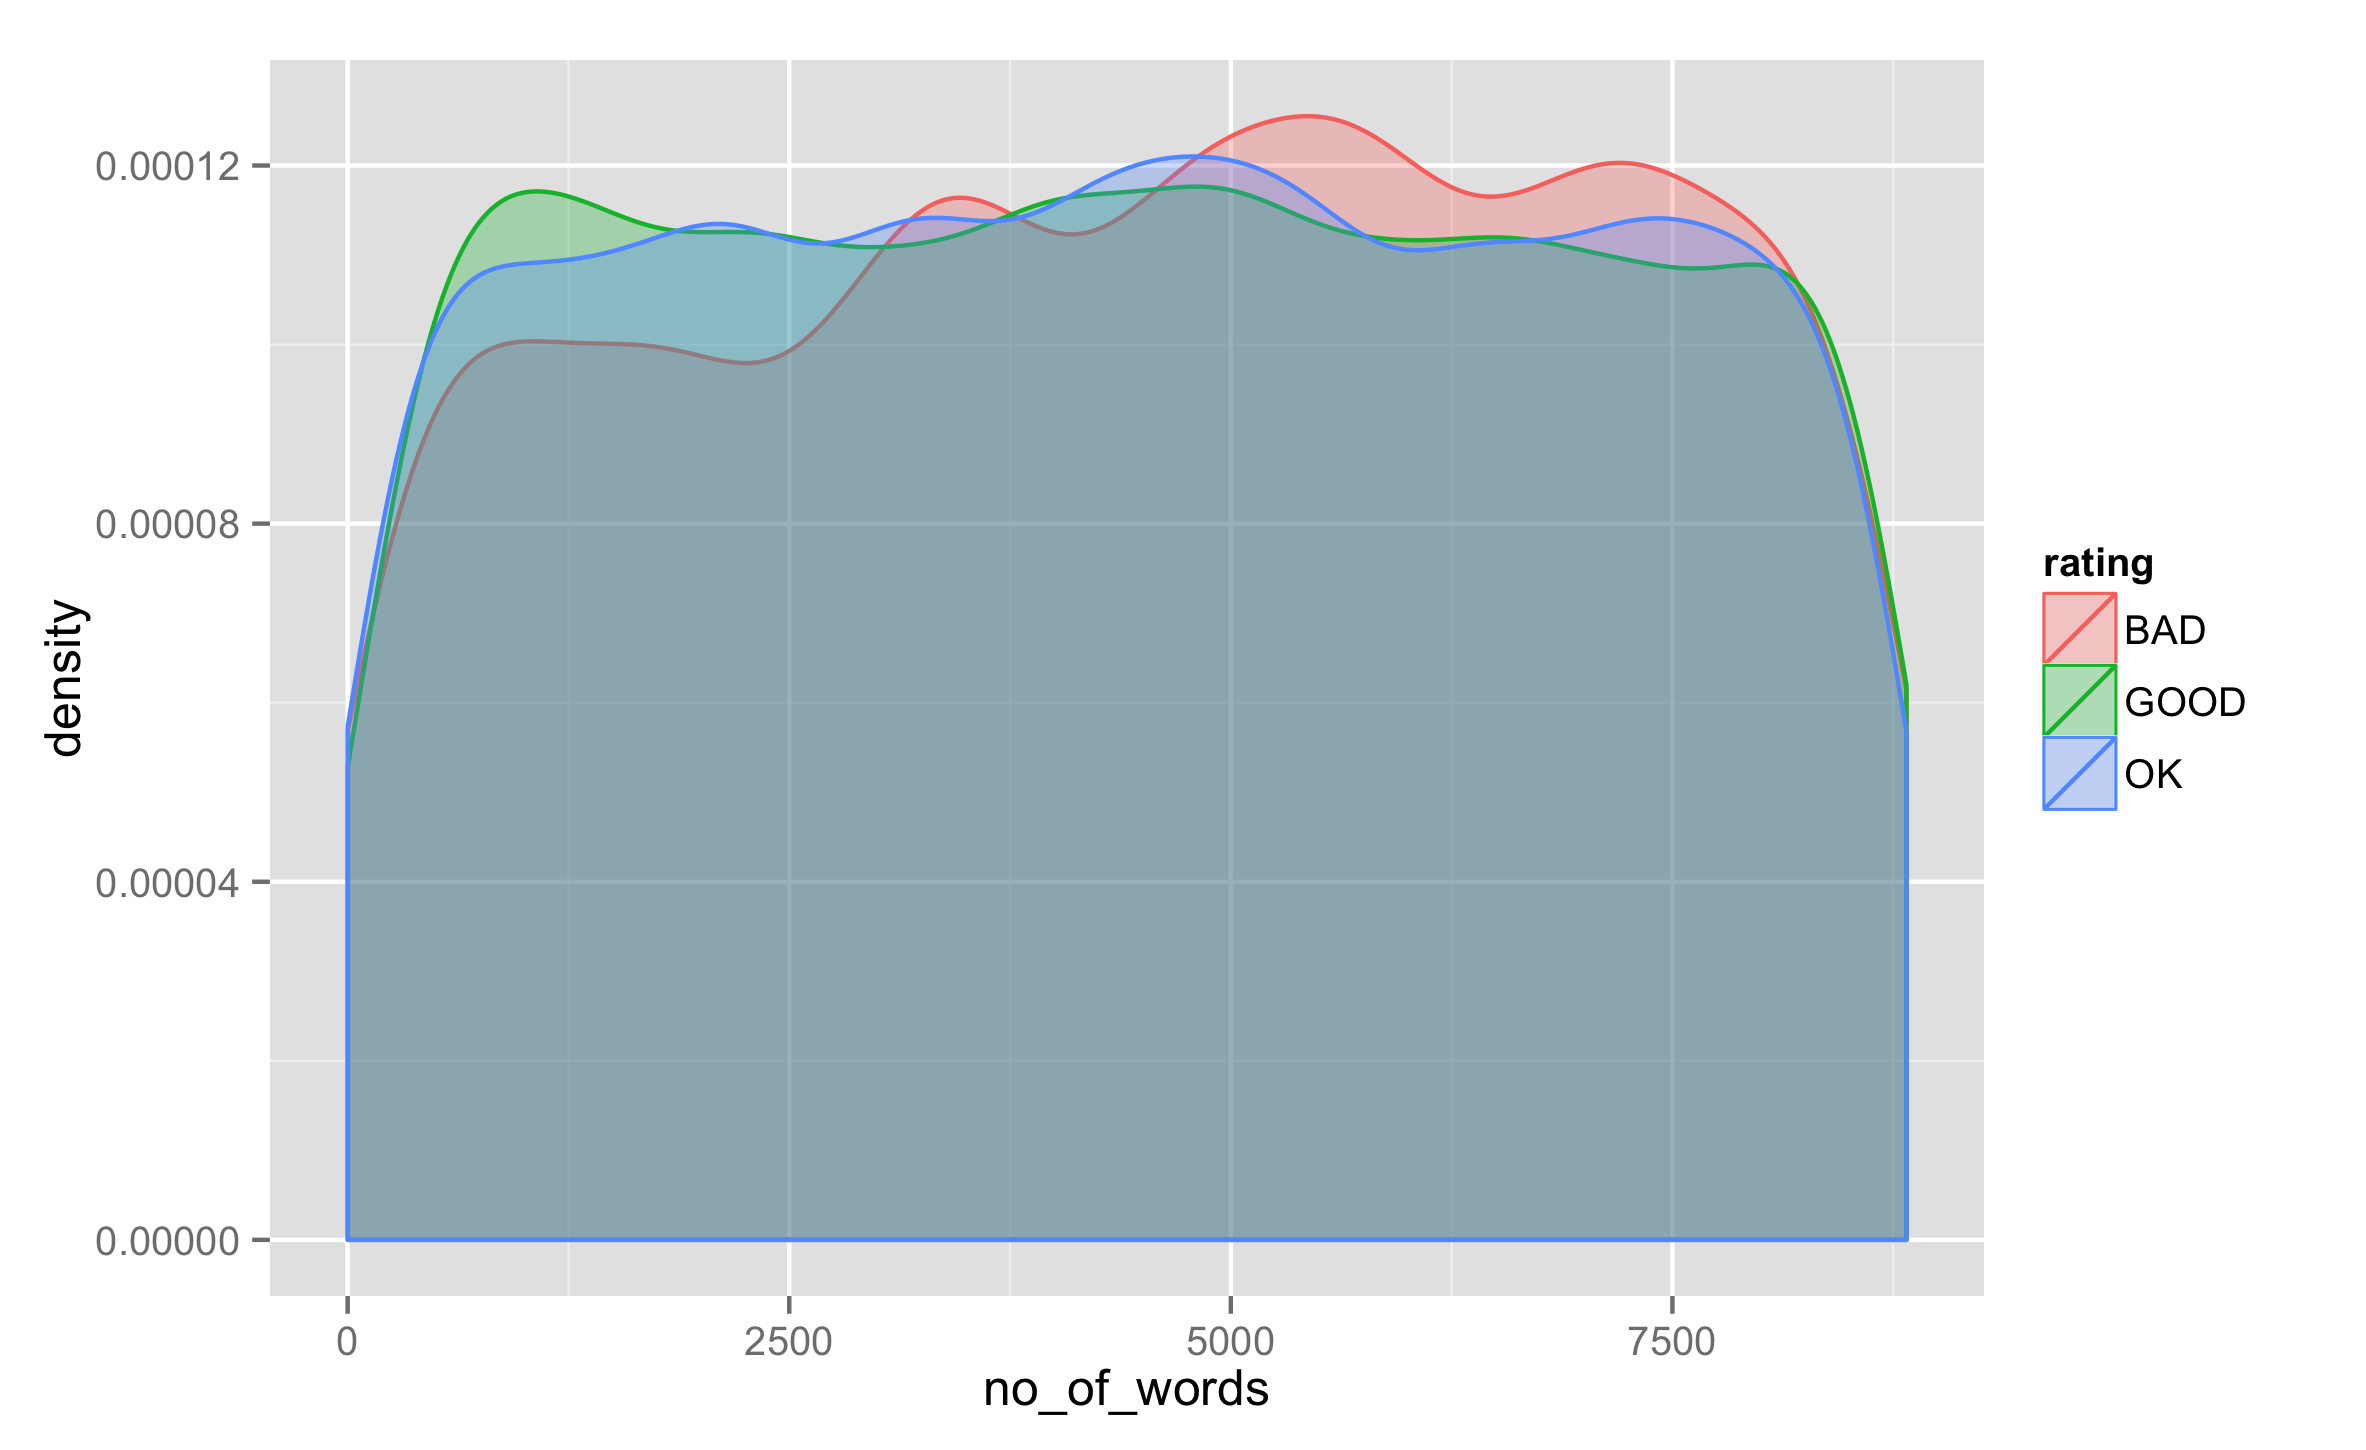
\includegraphics[width=6cm]{./plots/no-of-words.png} }}%
    \caption{2 Figures side by side}%
    \label{fig:example}%
\end{figure}


Unique number of food entities

\begin{figure}[h]
  \begin{center}
    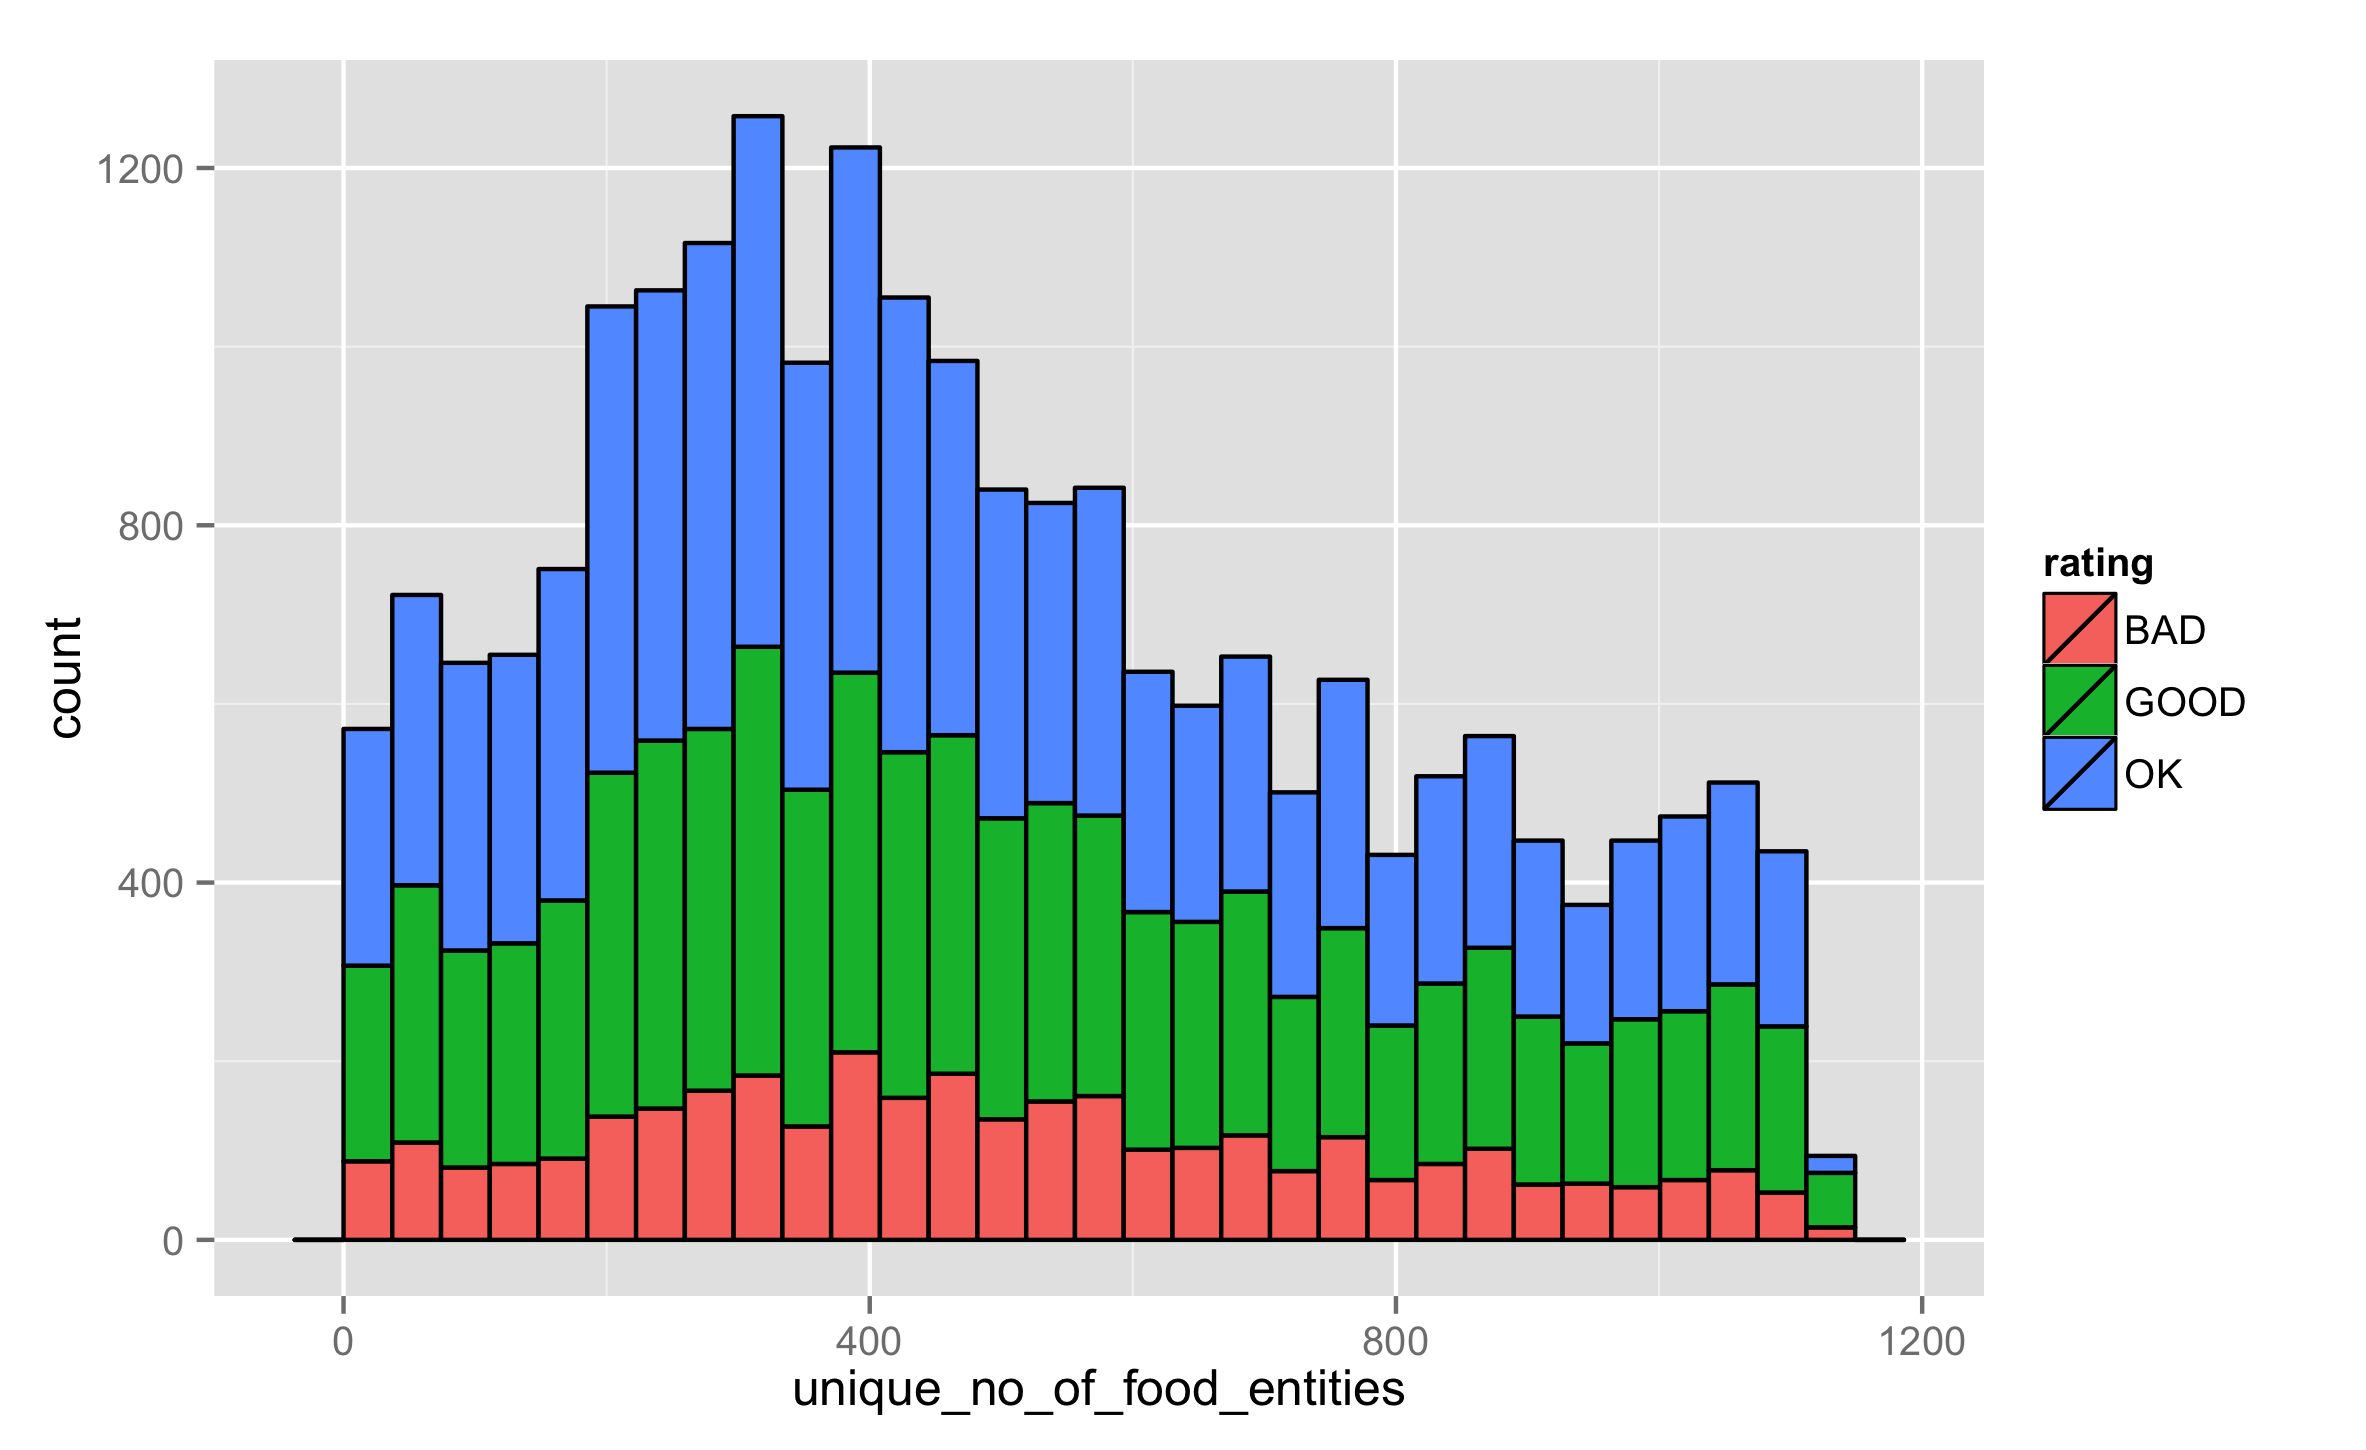
\includegraphics[scale=0.1]{./plots/unique-no-of-food-entities.png}
    \label{fig:}
    \caption{}
  \end{center}
\end{figure}




\section{Experiments and Results}
\section{Discussion and Conclussions}

\subsubsection*{References}


\small{
[1] Limin Yao, Sebastian Riedel \& Andrew McCallum. (2013) 
Universal Schema for Entity Type Prediction. 
{\it Workshop on Automated Knowledge Base Construction at CIKM }

[2] Arvind Neelakantan \& Michael Collins. (2014)
Learning Dictionaries for Named Entity Recognition using Minimal Supervision. 
}

\end{document}
